%% silkpage_coat_of_arms_01.tex — Mathematical Silk Heraldry
%%
%% SilkPage rendered as grand arms:
%% - silk canopy built from periodic curves
%% - page and markup as the central escutcheon
%% - lambda and arithmetic progression as executable grammar
%% - complex-plane spiral for temporal algebra
%% - mathematically generated ornament in the spirit of geometric elegance
%%
%% compile: xelatex silkpage_coat_of_arms_01.tex

\documentclass[border=24pt]{standalone}
\usepackage{tikz}
\usepackage{fontspec}
\usepackage{xcolor}
\usetikzlibrary{calc}

\newfontfamily\latinfont[
  Path=/System/Library/Fonts/,
  Ligatures=TeX, Kerning=On, Numbers=OldStyle
]{SFNS.ttf}

\definecolor{silkgreen}{HTML}{566E41}
\definecolor{deepgreen}{HTML}{26630A}
\definecolor{sage}{HTML}{DCE5D4}
\definecolor{maroon}{HTML}{57160F}
\definecolor{orange}{HTML}{E97E00}
\definecolor{paper}{HTML}{FFFFFF}
\definecolor{lightgray}{HTML}{DDDDDD}
\definecolor{ink}{HTML}{333333}
\definecolor{linkblue}{HTML}{335588}

\pagecolor{paper}

\begin{document}
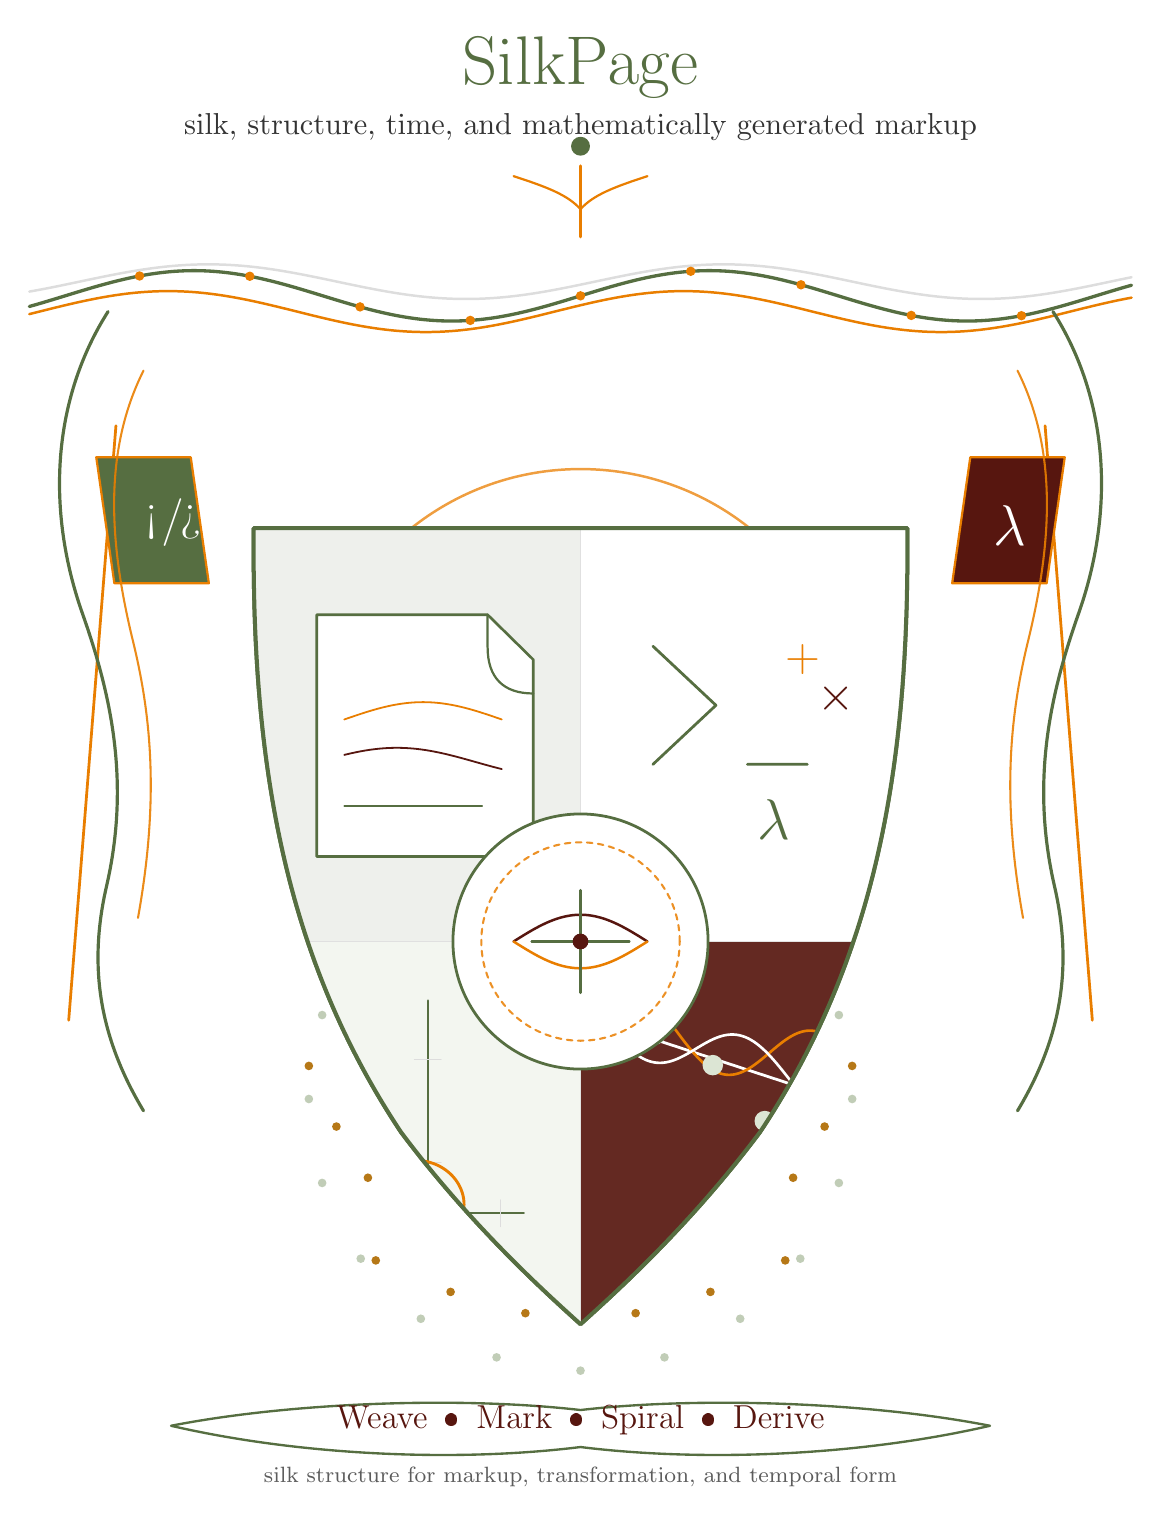
\begin{tikzpicture}[x=1cm,y=1cm,line cap=round,line join=round]

  %% title
  \node[font=\latinfont\fontsize{38pt}{40pt}\selectfont, text=silkgreen] at (0,13.1) {SilkPage};
  \node[font=\latinfont\fontsize{11pt}{13pt}\selectfont, text=ink] at (0,12.35)
    {silk, structure, time, and mathematically generated markup};

  %% top finial
  \draw[orange, line width=1.1pt] (0,11.85) -- (0,10.95);
  \fill[silkgreen] (0,12.1) circle (0.12);
  \draw[orange, line width=0.8pt]
    (-0.85,11.72) .. controls (-0.42,11.58) and (-0.16,11.48) .. (0,11.3)
    (0.85,11.72) .. controls (0.42,11.58) and (0.16,11.48) .. (0,11.3);

  %% silk canopy from periodic curves
  \draw[silkgreen, line width=1.2pt, samples=180, smooth, domain=-7:7]
    plot(\x, {10.2 + 0.32*sin(55*\x)});
  \draw[orange, line width=0.9pt, samples=180, smooth, domain=-7:7]
    plot(\x, {10.0 + 0.26*sin(55*\x + 18)});
  \draw[lightgray, line width=0.9pt, samples=180, smooth, domain=-7:7]
    plot(\x, {10.38 + 0.22*sin(55*\x - 10)});
  \foreach \x in {-5.6,-4.2,-2.8,-1.4,0,1.4,2.8,4.2,5.6} {
    \fill[orange] (\x,{10.2 + 0.32*sin(55*\x)}) circle (0.06);
  }

  %% side standards
  \draw[orange, line width=1.0pt] (-5.9,8.55) -- (-6.5,1.0);
  \draw[orange, line width=1.0pt] (5.9,8.55) -- (6.5,1.0);
  \fill[silkgreen] (-6.15,8.15) -- (-4.95,8.15) -- (-4.72,6.55) -- (-5.92,6.55) -- cycle;
  \fill[maroon] (6.15,8.15) -- (4.95,8.15) -- (4.72,6.55) -- (5.92,6.55) -- cycle;
  \draw[orange, line width=0.8pt] (-6.15,8.15) -- (-4.95,8.15) -- (-4.72,6.55) -- (-5.92,6.55) -- cycle;
  \draw[orange, line width=0.8pt] (6.15,8.15) -- (4.95,8.15) -- (4.72,6.55) -- (5.92,6.55) -- cycle;
  \node[font=\latinfont\fontsize{18pt}{18pt}\selectfont, text=paper] at (-5.45,7.32) {<};
  \node[font=\latinfont\fontsize{18pt}{18pt}\selectfont, text=paper] at (-5.18,7.32) {/};
  \node[font=\latinfont\fontsize{18pt}{18pt}\selectfont, text=paper] at (-4.95,7.32) {>};
  \node[font=\latinfont\fontsize{22pt}{22pt}\selectfont, text=paper] at (5.45,7.28) {$\lambda$};

  %% outer pavilion curtains
  \draw[silkgreen, line width=1.15pt]
    (-6.0,10.0) .. controls (-6.7,8.9) and (-6.8,7.5) .. (-6.32,6.15)
              .. controls (-5.95,5.1) and (-5.72,4.0) .. (-6.02,2.7)
              .. controls (-6.25,1.7) and (-6.12,0.8) .. (-5.55,-0.15);
  \draw[silkgreen, line width=1.15pt]
    (6.0,10.0) .. controls (6.7,8.9) and (6.8,7.5) .. (6.32,6.15)
             .. controls (5.95,5.1) and (5.72,4.0) .. (6.02,2.7)
             .. controls (6.25,1.7) and (6.12,0.8) .. (5.55,-0.15);
  \draw[orange, line width=0.75pt, opacity=0.9]
    (-5.55,9.25) .. controls (-6.05,8.25) and (-6.0,7.1) .. (-5.68,5.8)
               .. controls (-5.45,4.85) and (-5.35,3.8) .. (-5.62,2.3);
  \draw[orange, line width=0.75pt, opacity=0.9]
    (5.55,9.25) .. controls (6.05,8.25) and (6.0,7.1) .. (5.68,5.8)
              .. controls (5.45,4.85) and (5.35,3.8) .. (5.62,2.3);

  %% orbital collar
  \draw[orange, line width=0.9pt, opacity=0.75] (0,4.55) circle (3.45);
  \foreach \a in {0,18,...,342} {
    \fill[sage!80!silkgreen] (\a:3.45) circle (0.055);
  }

  %% main shield
  \path[fill=paper, draw=silkgreen, line width=1.45pt]
    (-4.15,7.25)
      .. controls (-4.18,4.1) and (-3.7,1.72) ..
    (-2.28,-0.42)
      .. controls (-1.38,-1.62) and (-0.42,-2.48) ..
    (0,-2.86)
      .. controls (0.42,-2.48) and (1.38,-1.62) ..
    (2.28,-0.42)
      .. controls (3.7,1.72) and (4.18,4.1) ..
    (4.15,7.25) -- cycle;

  \begin{scope}
  \clip
    (-4.15,7.25)
      .. controls (-4.18,4.1) and (-3.7,1.72) ..
    (-2.28,-0.42)
      .. controls (-1.38,-1.62) and (-0.42,-2.48) ..
    (0,-2.86)
      .. controls (0.42,-2.48) and (1.38,-1.62) ..
    (2.28,-0.42)
      .. controls (3.7,1.72) and (4.18,4.1) ..
    (4.15,7.25) -- cycle;

  %% shield fields
  \fill[silkgreen!10] (-4.3,2.0) rectangle (0.0,7.4);
  \fill[paper]        (0.0,2.0) rectangle (4.3,7.4);
  \fill[sage!35]      (-4.3,-3.0) rectangle (0.0,2.0);
  \fill[maroon!92]    (0.0,-3.0) rectangle (4.3,2.0);

  \draw[lightgray, line width=0.45pt, opacity=0.8] (-4.15,2.0) -- (4.15,2.0);
  \draw[lightgray, line width=0.45pt, opacity=0.8] (0,7.25) -- (0,-2.86);

  %% upper-left: folded page + woven lines
  \path[fill=paper, draw=silkgreen, line width=0.95pt]
    (-3.35,6.15) -- (-1.18,6.15) -- (-0.6,5.58) -- (-0.6,3.08)
    -- (-3.35,3.08) -- cycle;
  \draw[silkgreen, line width=0.8pt] (-1.18,6.15) -- (-1.18,5.74)
                                      .. controls (-1.18,5.35) and (-0.98,5.15) .. (-0.6,5.15);
  \draw[orange, line width=0.65pt, samples=80, smooth, domain=-3.0:-1.0]
    plot(\x, {4.82 + 0.22*sin(180*(\x+3.0)/2.0)});
  \draw[maroon, line width=0.65pt, samples=80, smooth, domain=-3.0:-1.0]
    plot(\x, {4.28 + 0.18*sin(180*(\x+3.0)/2.0 + 30)});
  \draw[silkgreen, line width=0.65pt] (-3.0,3.72) -- (-1.25,3.72);

  %% upper-right: markup and arithmetic derivation
  \draw[silkgreen, line width=1.0pt]
    (0.92,5.75) -- (1.72,5.0) -- (0.92,4.25)
    (2.12,4.25) -- (2.88,4.25);
  \node[font=\latinfont\fontsize{17pt}{17pt}\selectfont, text=orange] at (2.82,5.58) {+};
  \node[font=\latinfont\fontsize{17pt}{17pt}\selectfont, text=maroon] at (3.24,5.08) {$\times$};
  \node[font=\latinfont\fontsize{20pt}{20pt}\selectfont, text=silkgreen] at (2.45,3.55) {$\lambda$};

  %% lower-left: complex plane and logarithmic spiral
  \draw[silkgreen, line width=0.85pt] (-3.15,-1.45) -- (-0.72,-1.45);
  \draw[silkgreen, line width=0.85pt] (-1.94,-2.5) -- (-1.94,1.25);
  \foreach \x in {-2.86,-2.4,-1.48,-1.02} {
    \draw[lightgray, line width=0.35pt] (\x,-1.62) -- (\x,-1.28);
  }
  \foreach \y in {-2.1,-0.8,0.5} {
    \draw[lightgray, line width=0.35pt] (-2.11,\y) -- (-1.77,\y);
  }
  \draw[orange, line width=1.05pt, samples=180, variable=\t, domain=0:510]
    plot ({-1.94 + 0.10*exp(\t/240)*cos(\t)},
          {-1.45 + 0.10*exp(\t/240)*sin(\t)});
  \fill[maroon] (-1.94,-1.45) circle (0.06);

  %% lower-right: temporal braid / spiral time
  \draw[paper, line width=1.0pt, samples=120, smooth, domain=0.35:3.25]
    plot(\x, {0.95 - 0.95*(\x-0.35)/(2.9)});
  \draw[orange, line width=0.95pt, samples=140, smooth, domain=0.55:3.35]
    plot(\x, {1.05 - 0.70*(\x-0.55)/(2.8) + 0.42*sin(150*\x)});
  \draw[paper, line width=0.95pt, samples=140, smooth, domain=0.55:3.35]
    plot(\x, {0.95 - 0.95*(\x-0.55)/(2.8) + 0.36*sin(150*\x + 140)});
  \foreach \x/\y in {0.95/0.82,1.68/0.43,2.34/-0.28,2.88/-1.0} {
    \fill[sage] (\x,\y) circle (0.13);
  }

  %% center roundel: weave, lambda, and page eye
  \fill[paper] (0,2.0) circle (1.62);
  \draw[silkgreen, line width=1.0pt] (0,2.0) circle (1.62);
  \draw[orange, line width=0.75pt, opacity=0.85, dash pattern=on 2pt off 2pt] (0,2.0) circle (1.26);
  \draw[maroon, line width=0.9pt, samples=70, smooth, domain=-0.85:0.85]
    plot(\x, {2.0 + 0.34*cos(180*\x/1.7)});
  \draw[orange, line width=0.9pt, samples=70, smooth, domain=-0.85:0.85]
    plot(\x, {2.0 - 0.34*cos(180*\x/1.7)});
  \draw[silkgreen, line width=1.0pt]
    (-0.62,2.0) -- (0.62,2.0)
    (0,1.35) -- (0,2.65);
  \fill[maroon] (0,2.0) circle (0.1);

  \end{scope}

  %% redraw shield border
  \path[fill=none, draw=silkgreen, line width=1.45pt]
    (-4.15,7.25)
      .. controls (-4.18,4.1) and (-3.7,1.72) ..
    (-2.28,-0.42)
      .. controls (-1.38,-1.62) and (-0.42,-2.48) ..
    (0,-2.86)
      .. controls (0.42,-2.48) and (1.38,-1.62) ..
    (2.28,-0.42)
      .. controls (3.7,1.72) and (4.18,4.1) ..
    (4.15,7.25) -- cycle;

  %% small geometric satellites inspired by mathematical ornament
  \foreach \x/\y in {-3.45/0.42,-3.1/-0.35,-2.7/-1.0,3.45/0.42,3.1/-0.35,2.7/-1.0,
                     -2.6/-2.05,-1.65/-2.45,-0.7/-2.72,0.7/-2.72,1.65/-2.45,2.6/-2.05} {
    \fill[orange!65!silkgreen] (\x,\y) circle (0.055);
  }

  %% motto ribbon
  \path[fill=paper, draw=silkgreen, line width=0.85pt]
    (-5.2,-4.15)
      .. controls (-3.6,-4.52) and (-1.62,-4.62) ..
    (0,-4.42)
      .. controls (1.62,-4.62) and (3.6,-4.52) ..
    (5.2,-4.15)
      .. controls (3.72,-3.86) and (1.58,-3.77) ..
    (0,-3.95)
      .. controls (-1.58,-3.77) and (-3.72,-3.86) ..
    (-5.2,-4.15) -- cycle;
  \node[font=\latinfont\fontsize{11.5pt}{12.5pt}\selectfont, text=maroon] at (0,-4.08)
    {Weave \,•\, Mark \,•\, Spiral \,•\, Derive};
  \node[font=\latinfont\fontsize{8.2pt}{9.6pt}\selectfont, text=ink, opacity=0.8] at (0,-4.8)
    {silk structure for markup, transformation, and temporal form};

\end{tikzpicture}
\end{document}
